%   Dylan Wright - dylan.wright@uky.edu
%   Casey O'kane - casey.okane@uky.edu
%   EE480 - Assignment 2: The Making Of An IDIOT
%   note.tex : Implementer's Note
%   Version:
%       02-14-2016 : initial
%	  03-06-2016 : Revised content slightly, added "General Approach" and 
%			      "Issues" subsection. Wrote a basic abstract  that may be
%				revised later. 
%	 03-09-2016: Continued to revise content. Added initial information for
%			     Verilog Module testing, General Approach, and the three
%			     subsections related to issues. Also created a general
%			     appendix. 
%      03-10-2016:

\documentclass[conference]{IEEEtran}
\usepackage{graphicx}
\usepackage{float}
\usepackage{verbatim}
\usepackage{adjustbox}

\begin{document}
\title{Assignment 2: The Making Of An IDIOT\\Implementor's Notes}
\author{\IEEEauthorblockN{Dylan Wright}
        \IEEEauthorblockA{dylan.wright@uky.edu}
        \IEEEauthorblockN{Casey O'Kane}
        \IEEEauthorblockA{casey.okane@uky.edu}}

\maketitle

\begin{abstract}
Goal of this assignment involved the implementation of the IDIOT instruction set
using the AIK assembler, the Verilog Hardware Design Language and detailed test
plan to exhaustively test the different components and logic of the design. 
\end{abstract}

\section{Testing}
\subsection{Instruction Set Architecture}
In order to test the IDIOT instruction set specification a test framework was
implemented. This framework is in the \texttt{IDIOT/} directory. The framework
consists of the following files:
\subsubsection{\texttt{aik.py}}
To automatically test files \texttt{aik.py} sends a PUSH request to the
AIK cgi program. The returned html page is parsed and each section is output.
The \texttt{.text} and \texttt{.data} sections are sent to stdout and the
assembler messages are sent to \texttt{stderr}. This method is not ideal, an
AIK executable would be preferable. Sample run:
\begin{verbatim}
 $ echo "file.idiot" | ./aik.py
\end{verbatim}
\subsubsection{\texttt{diss.py}}
To make test results human readable, \texttt{diss.py} disassembles a 
\texttt{.out} file (the \texttt{.text} and \texttt{.data} segment of the 
output of \texttt{aik.py}). The code is converted to binary and displayed in
tabular format. Sample run:
\begin{verbatim}
 $ echo "file.out" | ./diss.py
\end{verbatim}
\subsubsection{\texttt{test.sh}}
This file can be used to test each \texttt{.idiot} file in the \texttt{progs/}
directory. This script runs each file through AIK and compares the output to
the expected output. \texttt{.text} and \texttt{.data} segment expected
output should be placed in a file with the same name as the program and a 
\texttt{.expected.out} file extension. Expected assembler messages should
be placed in a file with a \texttt{.expected.err} extension. The test script
will report the number of passed, failed and possibly failed tests. This test
framework was adapted from a script provided by Dr. Jaromczyk in the Fall
2015 CS 441G: Compilers course. Sample run:
\begin{verbatim}
 $ ./test
\end{verbatim}

\subsection{Verilog Modules}
Every Verilog module included in the provided tarball has an associated
testbench file, as denoted by the *\_tb.v extension that is used for each
module. All of the tests can be run using the \texttt{test.sh} script in 
the verilog directory. 

\subsubsection{\texttt{alu\_tb.v}}
This testbench execises the ALU module defined in \texttt{alu.v} by reading
in test vectors and checking the ALU's output. The test vectors are in
\texttt{tests/aluXvector.vmem}, \texttt{tests/aluYvector.vmem},
\texttt{tests/aluZvector.vmem}, \texttt{tests/aluOpvector.vmem}. 

\subsubsection{\texttt{memory\_tb.v}}
This testbench exercises the memory module defined in \texttt{memory.v} by
setting each cell's value to its address. Next it checks that each cell's value
has not changed.

\subsubsection{\texttt{register\_file\_tb.v}}
This testbenc exercises the register file module defined in \texttt{register\_file.v} with the same methodology as the memory test bench.

\subsubsection{\texttt{proccesor\_tb.v}}
This testbench exercises the control logic and proccesor connections. It does
so by providing a reset and clock to the instantiated proccesor module (defined
in \texttt{proccesor.v}). The memory module is initialized with a vmem file. By
default this is \texttt{tests/proccesor/proccesor-test-non-trivial.vmem}. This
contains a non trivial program generated by \texttt{idiocc} and \texttt{aik}. 
This testbench is also used to run the other proccesor vmem tests by 
\texttt{test.sh}. \\

The other primary test vector for this testbench is
\texttt{tests/proccesor/proccesor-custom.vmem}. This contains a custom IDIOT
assembly program assembled using \texttt{aik}. This program performs a simple
loop. After that it executes the thusfar ALU instructions, squash, store, and
load. Then it ends. Because this program uses every instruction it produces 
nearly complete coverage. The output of covered for this program is included
as Documentation/covreport.txt

\subsection{Utilization of GTKWave}
GTKWave was used extensivly to debug timing issues with the control. It was 
helpful to see when signals were being changed. 


\section{General Approach}
Due to the complex nature of this assignment, the general approach 
first involved forming a top down design, a comprehensive finite
state machine (FSM) for the ISA instructions and then a far more specific
FSM. Diagrams were created for these designs and they can be 
found as \textbf{Figures 1, 2, 3, and 4} respectively in the \textbf{Appendix} 
of this report. 

One key decision that was made over the course of this project included 
the decision to select a Harvard Architecture as a model for the memory unit
rather than a Von Neumann model. The group ultimately decided to go 
with this method as it would allow them to simultaneously read or write
instructions to or from memory.This decision is reflected in the AIK 
specification that was created \texttt{IDIOT\_Specv} found in the \texttt{IDIOT}
directory of the provided tarball).

After constructing the top down design, the AIK specification
for the project was formed as \texttt{IDIOT\_Spec}. This specification primarily involved specifying IDIOT ISA 
instructions using the conventions discussed discussed in class, for example all
floating point instructions are actually system calls (or HALTs) which can be implemented as a special case of the jz instruction. 

Once the AIK specification was created, skeleton modules \texttt{alu.v, control.v,
memory.v, processor.v,} and \texttt{register\_file.v} followed. Initially these files were 
written with basic functionality and later expanded using a top level approach,
by then setting up \texttt{processor.v} and the completing the modules that it
instantiates. \texttt{signals.v} contains many of the signals that would be used  to communicate 
between devices along with a few global constants utilized throughout the 
Verilog code (the 16 bit register constant WORD for example).

Speaking more to \texttt{processor.v}, it instantiates the other necessary modules
and then uses one level sensitive  and two edge sensitive always blocks to 
simulate the processor. The specifics of these operations are detailed 
in the diagrams represented in the \textbf{Appendix} of these notes
 
After completing all of the mentioned modules, associated test benches were 
constructed as stated in \textbf{B. Verilog Modules} of the \textbf{Testing} portion
of these notes and issues wereresolved as they arose.
 


\section{Issues}
\subsection{Possible Errors}
We're still in the early stages of testing so there is the possibility of many things 
being incorrect. This is something that I will fill in with more detail as we 
further approach completion with the testing of the assignment.

Also, it might help to view the following \textbf{Notable Workarounds} section
of this section, that might be another location were a problem might arise.

\subsection{Notable Workarounds}
\subsubsection{Instruction Register Assignment}
In processor.v, when assigning to the instruction register, it was decided 
that rather than storing the value stored on the Bus, that the value stored
in the MDR should be used as the IR only reads from the MDR anyway.
\subsubsection{Control FSM Timing}
The original design for the finite state machine was much smaller than the 
final one present in the project. In order to amilliorate timing issues, a
number of state were expanded into either multiple states or lengthened. This 
was usually due to a register not latching in time or the bus not having the
right value. While this is not an ideal solution to the problem, it does work.

\appendix{Notable Diagrams}

\clearpage 
\section{Top Down Design}
\begin{figure}[!t]
\centering
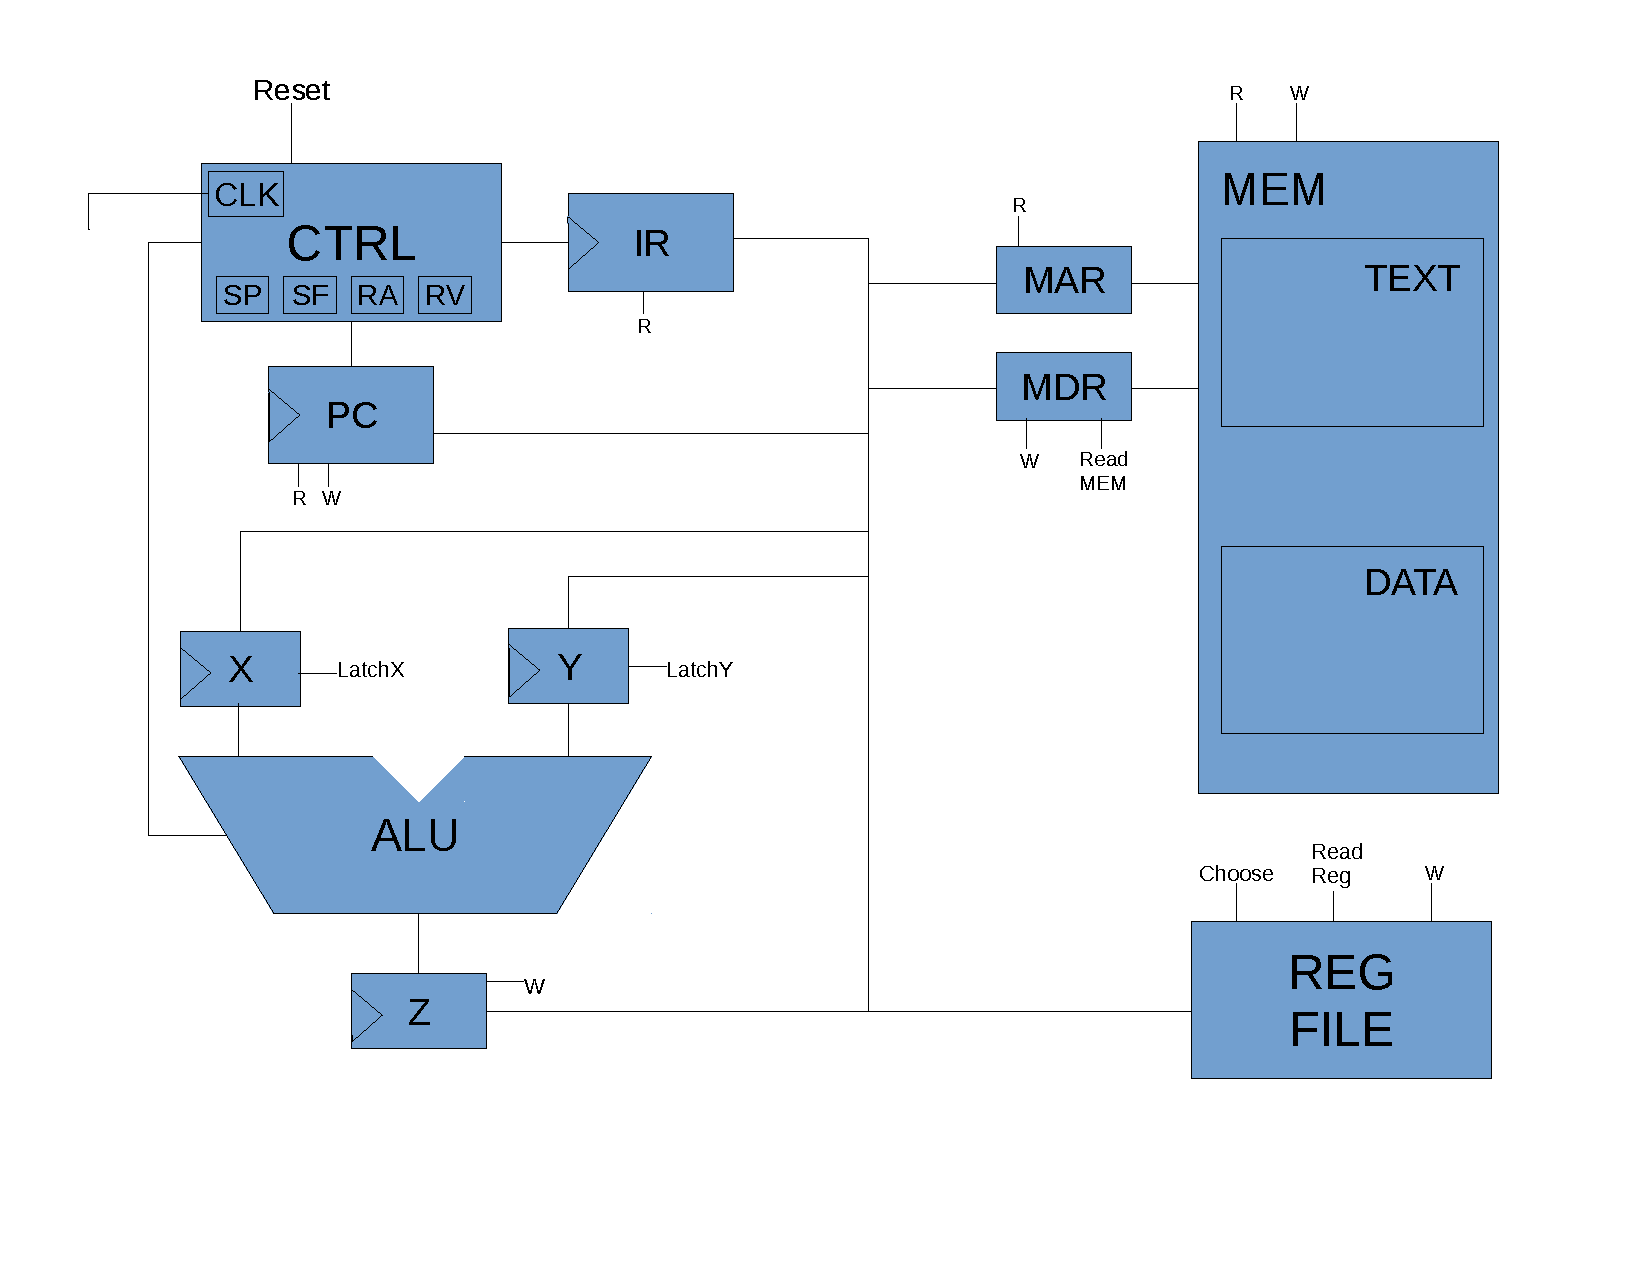
\includegraphics[width=\textwidth]{TopDownDesignDraftp1.pdf}
\caption{Top Down Design}
\label{fig_sim}
\end{figure}

\clearpage
\begin{figure}[!t]
\centering
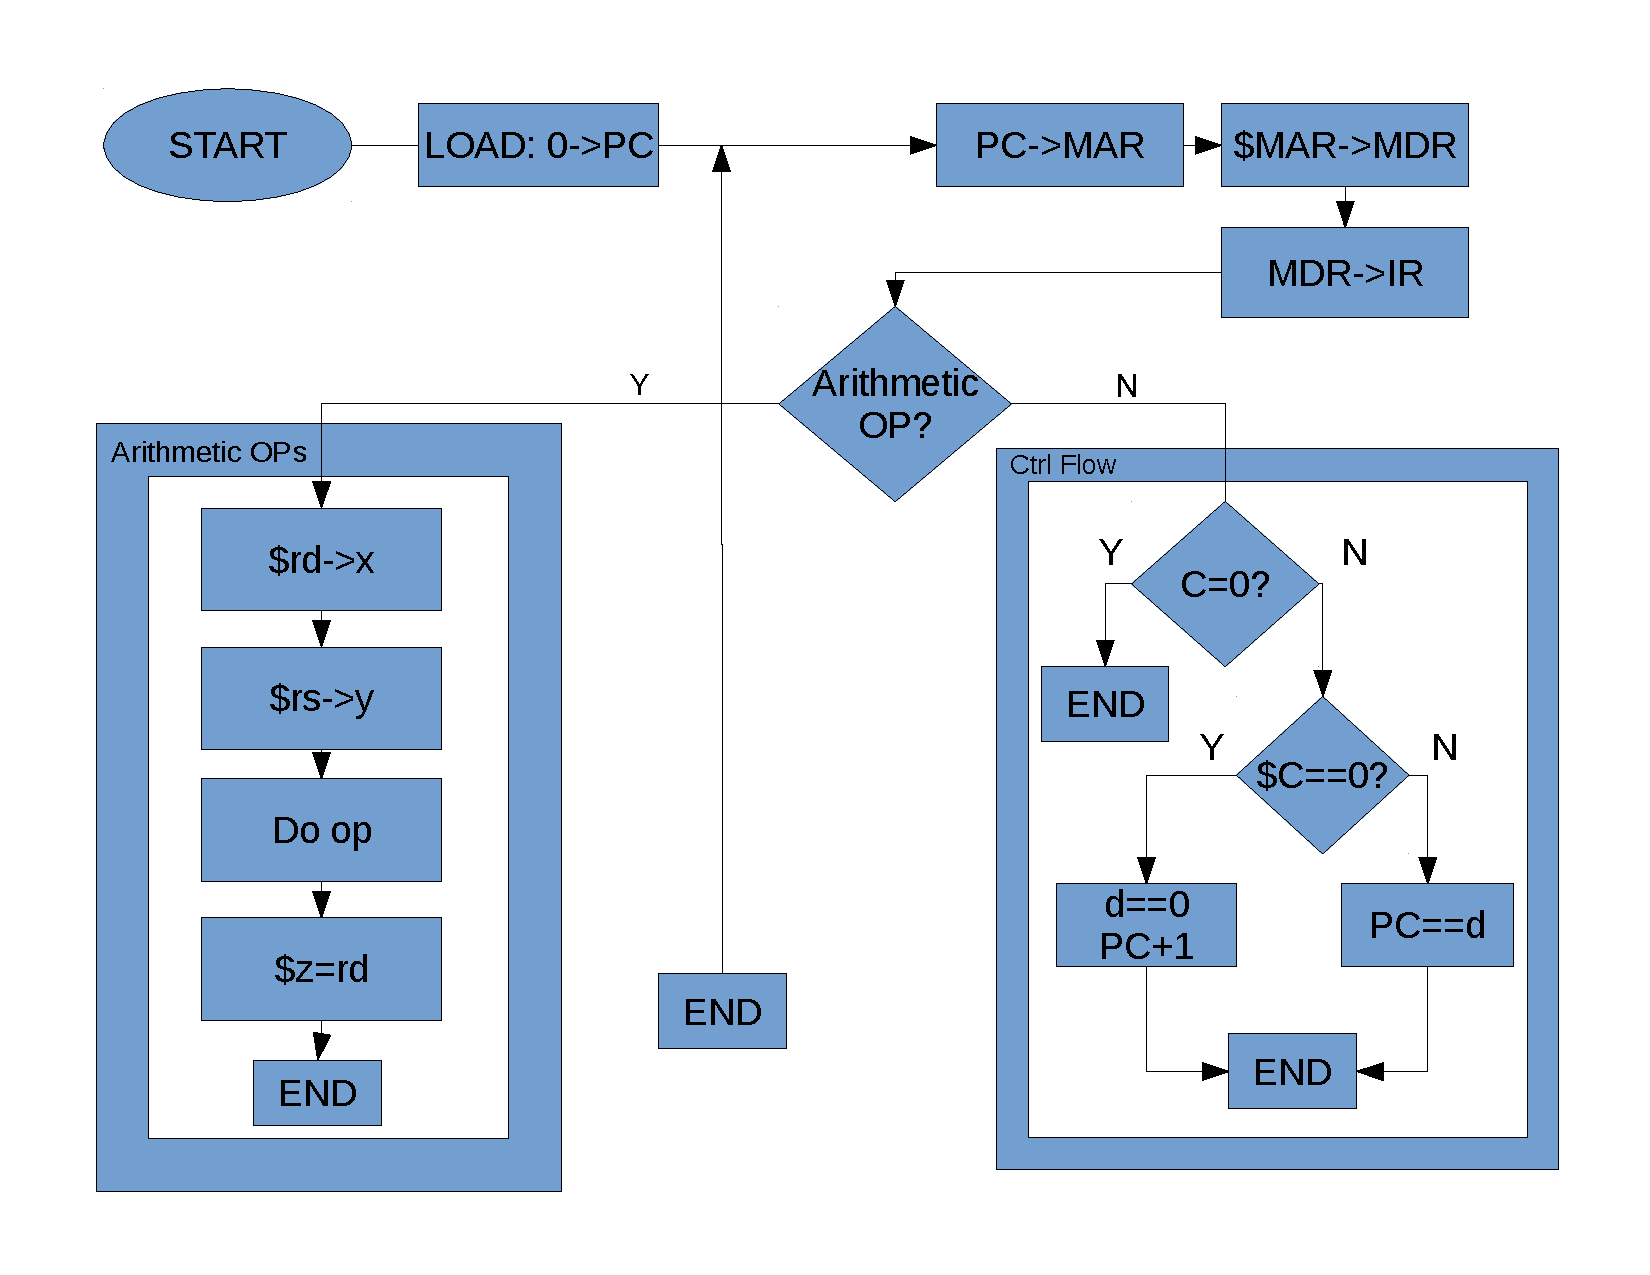
\includegraphics[width=\textwidth]{TopDownDesignDraftp2.pdf}
\caption{General FSM}
\label{fig_sim}
\end{figure}

\clearpage

\begin{figure}[!t]
\centering
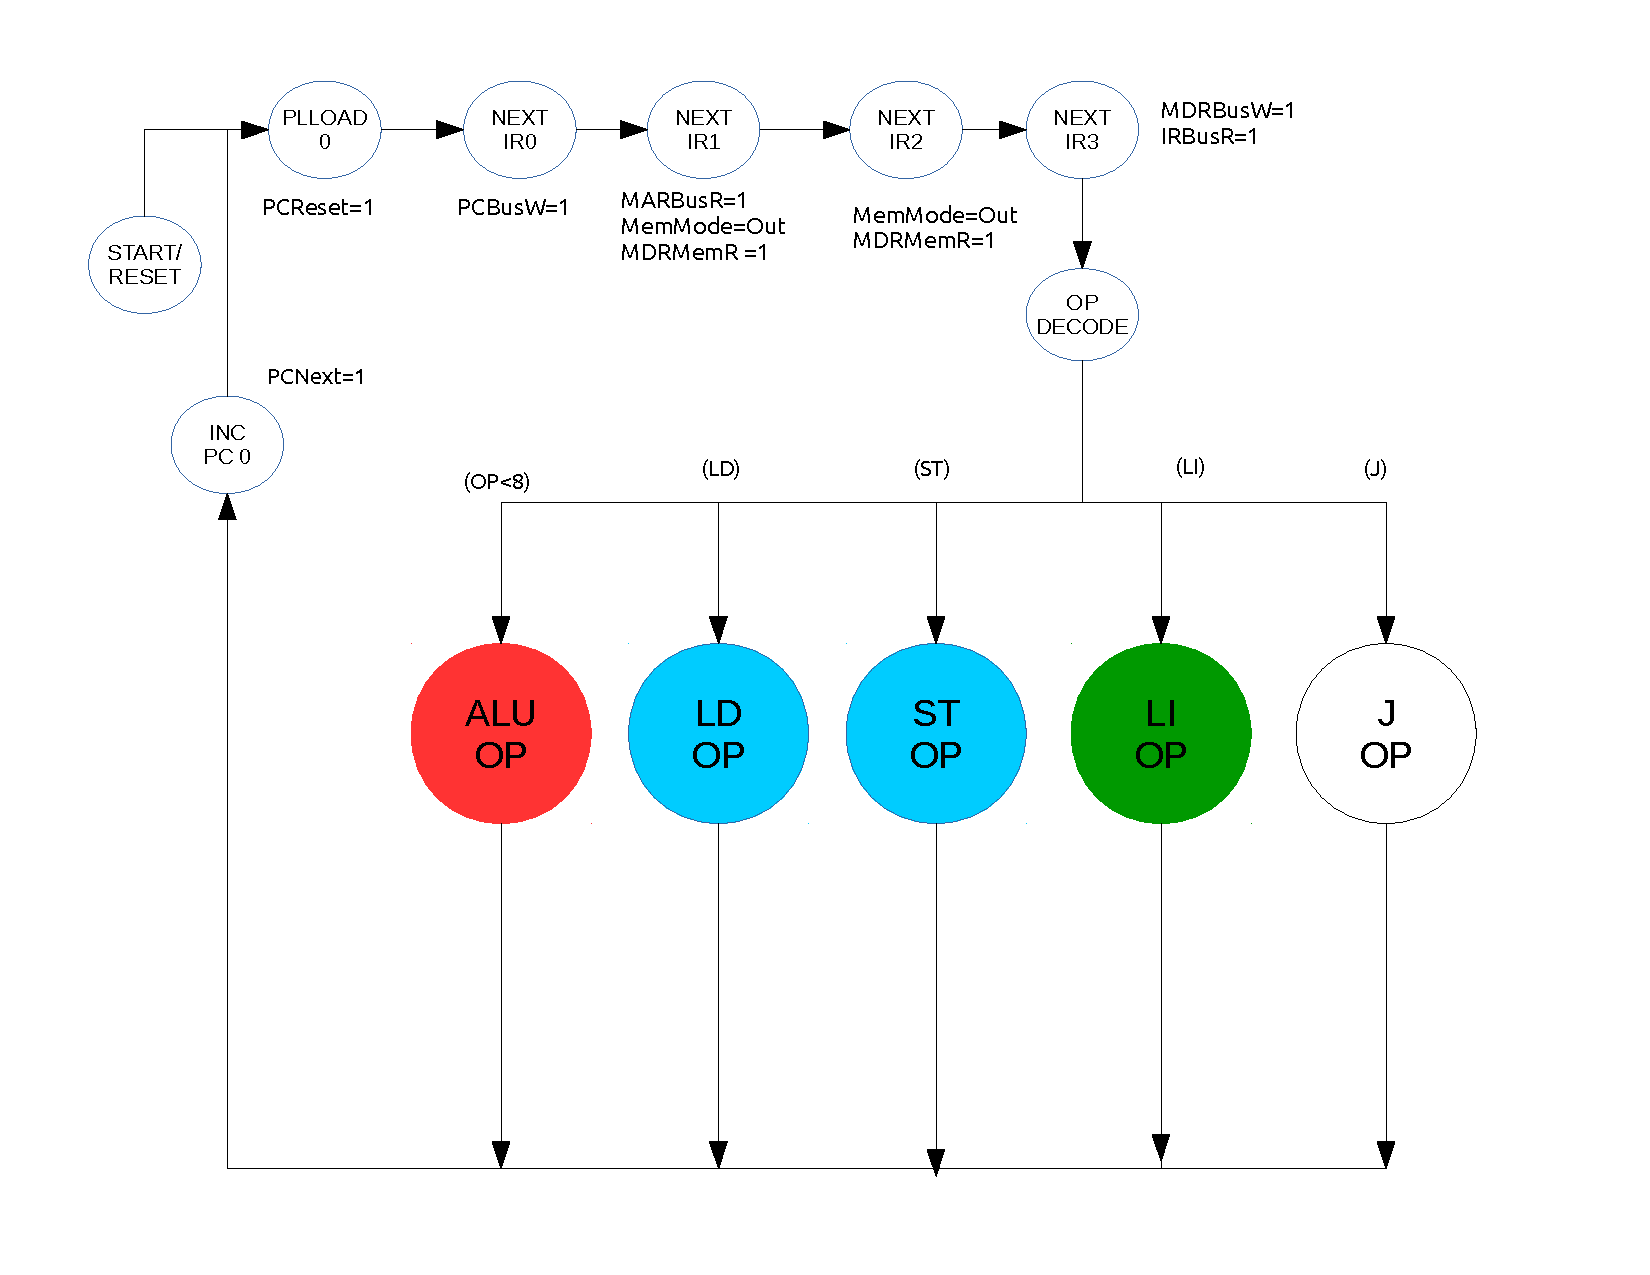
\includegraphics[width=\textwidth]{ControlFSMp1.pdf}
\caption{Detailed FSM without Jump Operations}
\label{fig_sim}
\end{figure}


\clearpage

\begin{figure}[!t]
\centering
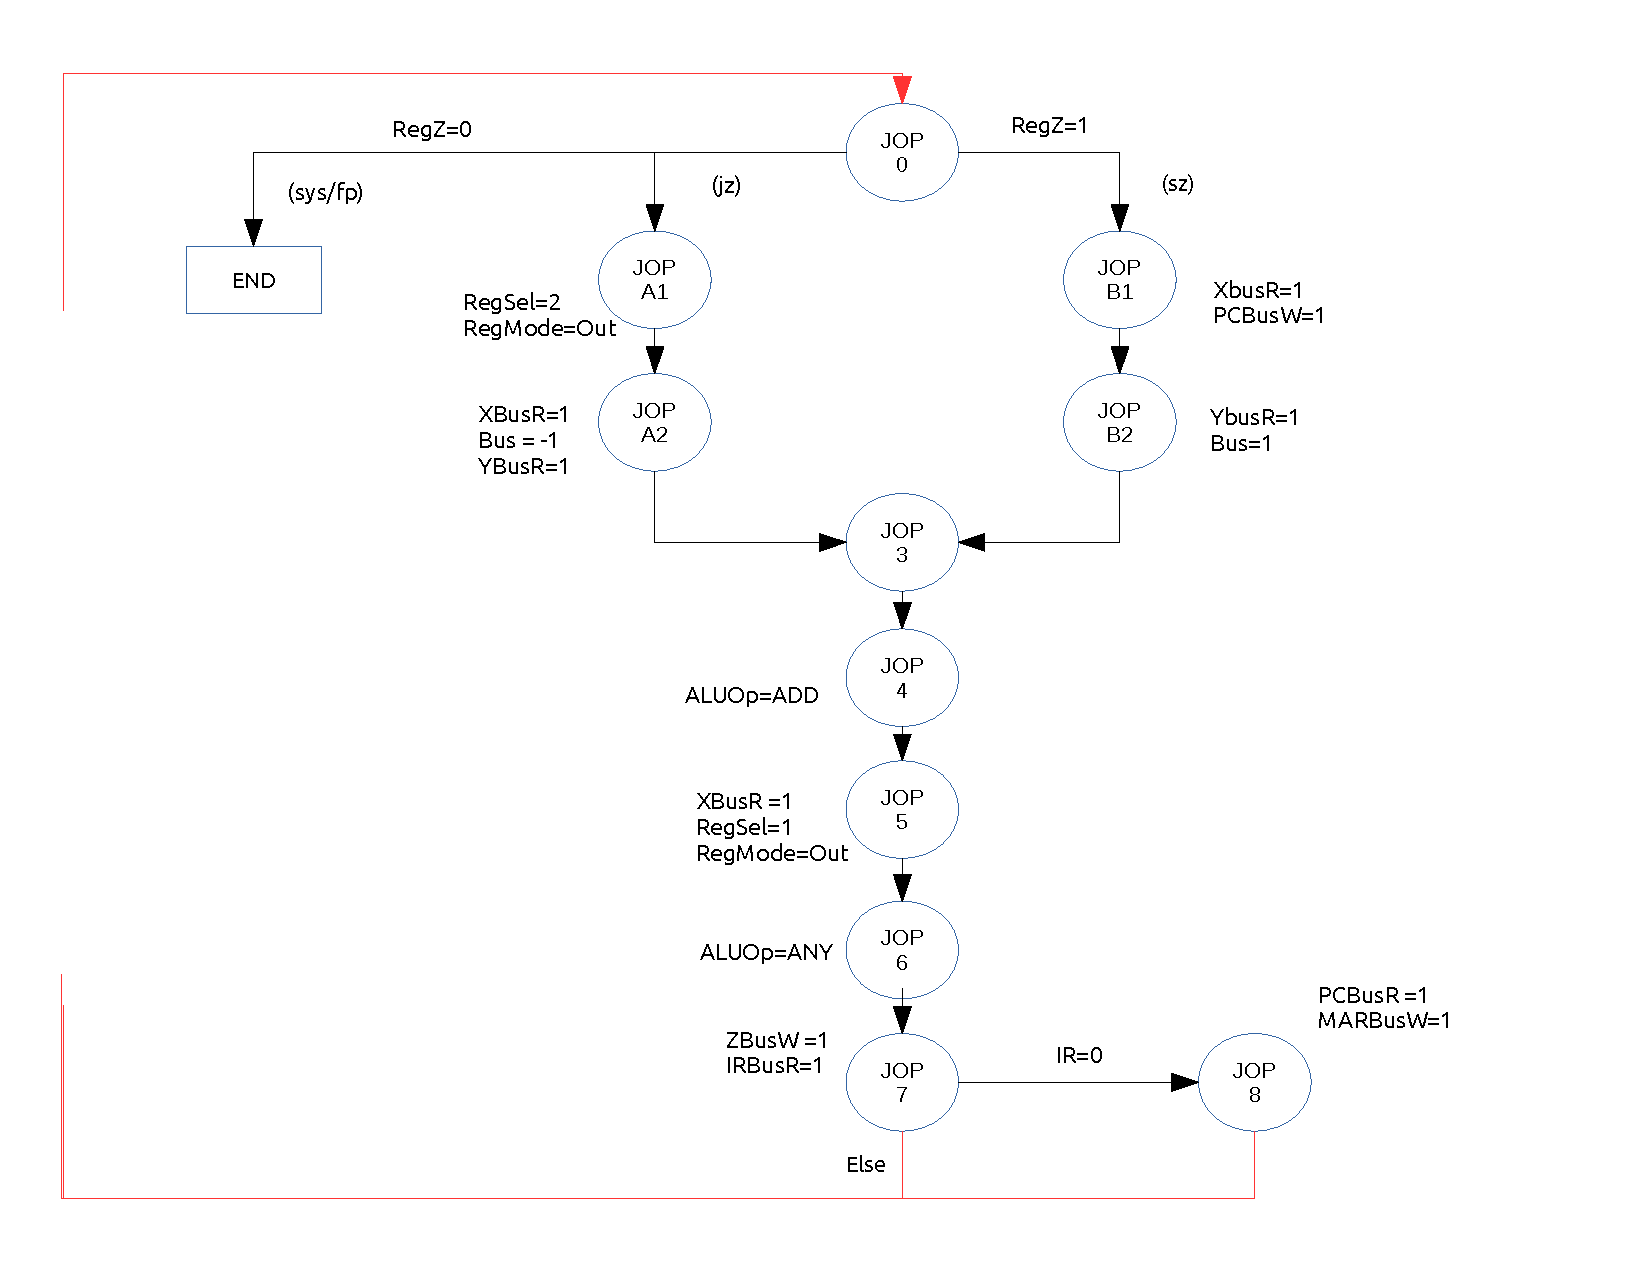
\includegraphics[width=\textwidth]{ControlFSMp2.pdf}
\caption{Detailed FSM with Jump Operations}
\label{fig_sim}
\end{figure}


\end{document}
